\documentclass[a4paper]{article}


\usepackage{CJK}
\usepackage{microtype}
%\usepackage{savesym}
%  \savesymbol{lambdabar}
\usepackage{newpxtext,eulerpx}
%  \restoresymbol{newpx}{lambdabar}
\usepackage[T1]{fontenc}
\usepackage[margin=2cm]{geometry}
%\usepackage{setspace}
\usepackage{amsmath}
%  \allowdisplaybreaks
\usepackage{bm}
\usepackage{dsfont}
%\usepackage{mathrsfs}
\usepackage{soul}
%\usepackage{tensor}
\usepackage{graphicx}
%\usepackage{booktabs}
%\usepackage{placeins}
%\usepackage{subcaption}
%\usepackage[caption=false]{subfig}  % revtex hates caption
\usepackage{hyperref}
  \hypersetup{
    colorlinks=true,
    linkcolor=BrickRed,
    filecolor=BrickRed,
    citecolor=BrickRed,
    urlcolor=RoyalBlue,
  }
\usepackage[numbers]{natbib}
\usepackage[dvipsnames]{xcolor}
\usepackage{comment}
  \newif\ifshow
  %\showtrue  % show
  \showfalse  % hide
  %
  \ifshow
    \includecomment{hide}
  \else
    \excludecomment{hide}
  \fi
\usepackage{tikz}
  \usetikzlibrary{positioning, fit, calc, arrows.meta}


\newcommand{\pmwd}{{\usefont{T1}{nova}{m}{sl}pmwd}}

\newcommand{\gkai}[1]{\begin{CJK*}{UTF8}{gkai}\raisebox{.1em}{(}#1\raisebox{.1em}{)}\end{CJK*}}

\renewcommand{\sectionautorefname}{Sec.}
\renewcommand{\subsectionautorefname}{Sec.}
\renewcommand{\subsubsectionautorefname}{Sec.}
\renewcommand{\appendixautorefname}{App.}
\renewcommand{\figureautorefname}{Fig.}
\newcommand{\subfigureautorefname}{\figureautorefname}

\DeclareMathOperator*{\E}{\mathds{E}}
\DeclareMathOperator{\tsum}{{\textstyle\sum}}
\newcommand{\1}{\mathds{1}}
\newcommand{\R}{\mathds{R}}
\newcommand{\Z}{\mathds{Z}}
\newcommand{\order}{\mathcal{O}}
\newcommand{\deltaD}{\delta^\textsc{d}}
\newcommand{\deltaK}{\delta^\textsc{k}}
\renewcommand{\d}{d}
\newcommand{\p}{\partial}
\newcommand{\cJ}{\mathcal{J}}
\newcommand{\cR}{\mathcal{R}}
\newcommand{\cL}{\mathcal{L}}
\newcommand{\cH}{\mathcal{H}}
\bmdefine{\vzero}{0}
\bmdefine{\vI}{I}
\bmdefine{\vnabla}{\nabla}
\bmdefine{\vtheta}{\theta}  % parameters
\bmdefine{\vomega}{\omega}  % white noise modes
\bmdefine{\vk}{k}  % wavevectors
\bmdefine{\vn}{n}  % wavevector indices
\bmdefine{\vm}{m}  % grid point indices
\bmdefine{\vj}{j}  % integer indices
\bmdefine{\vx}{x}  % comoving and canonical coordinates
\bmdefine{\vq}{q}  % Lagrangian coordinates
\bmdefine{\vs}{s}  % displacements
\bmdefine{\vp}{p}  % canonical momenta
\bmdefine{\va}{a}  % accelerations
\bmdefine{\vz}{z}  % states
\bmdefine{\vf}{f}
\bmdefine{\vF}{F}
\bmdefine{\vvarphi}{\varphi}
\newcommand{\As}{A_\mathrm{s}}
\newcommand{\ns}{n_\mathrm{s}}
\newcommand{\Omegam}{\Omega_\mathrm{m}}
\newcommand{\Omegab}{\Omega_\mathrm{b}}
\newcommand{\Mpc}{\mathrm{Mpc}}
\newcommand{\ic}{\mathrm{i}}
\newcommand{\knyq}{k_\mathrm{Nyq}}
\newcommand{\kfun}{k_\mathrm{fun}}

\newcommand{\GPU}{NVIDIA A100 80GB SXM4}

\newcommand{\YL}[1]{\textcolor{Bittersweet}{#1}}



\begin{document}



\title{Patching Particle-Particle Particle-Mesh Method}


\author{Yin Li \gkai{李寅}}


\date{2022-12}


\maketitle



\begin{abstract}
Adding the PP compensation to the PM force.
\end{abstract}



\section{Introduction}


\section{Methods}


\subsection{Particle-Mesh Force}


\YL{Describe briefly PM (and our corrections) here. Also introduce
possible filter below. Explain that we are not doing splitting the
usual way.}


\subsubsection{Partial Sum}

In a periodic box of size $L_1 \times \cdots \times L_d$ in $\R^d$,
Poisson's equation,
%
\begin{equation}
\nabla^2 u = f,
\label{Poisson}
\end{equation}
%
becomes
%
\begin{equation}
- k_\vn^2 u(\vk_\vn) = f(\vk_\vn),
\end{equation}
%
in Fourier space, with discretized wavevectors $\vk_\vn \triangleq (2\pi
n_1 / L_1, \cdots, 2\pi n_d / L_d )^\intercal$ and $n_i \in \Z$.
And the force $- \vnabla u$ becomes $i \vk_\vn f / k_\vn^2$.
When \eqref{Poisson} is further discretized by a $N_1 \times \cdots
\times N_d$ mesh of cell size $l$, with $\vx_\vm \triangleq (m_1 l,
\cdots, m_d l)^\intercal$ and $m_i \in \Z/N_i\Z$, $\vk_\vn$ is also
periodic with $n_i \in \Z/N_i\Z$.

At finite resolution, the bandwidth is truncated at the Nyquist
frequency $\knyq = \pi / l$.
In 1D, the partial sum is equivalent to a convolution by (the Dirichlet
kernel)
%
\begin{align}
\frac1{2 L} \Bigg(
  \sum_{n=-\lfloor\frac{N}2\rfloor}^{\lfloor\frac{N}2\rfloor}
  + \sum_{n=-\lfloor\frac{N-1}2\rfloor}^{\lfloor\frac{N-1}2\rfloor}
\Bigg) e^{i k_n x}
%
&= \frac{
  \sin \bigl[
    \bigl( \bigl\lfloor\frac{N}2\bigr\rfloor + \frac12 \bigr) \kfun x
  \bigr]
  + \sin \bigl[
    \bigl( \bigl\lfloor\frac{N-1}2\bigr\rfloor + \frac12 \bigr) \kfun x
  \bigr]
}{2 \sin \bigl( \frac12 \kfun x \bigr) L} \nonumber\\
%
&= \frac{\sin \bigl( \knyq x \bigr)}
        {\sin \bigl( \frac12 \kfun x \bigr) L}
\cdot \begin{cases}
  \cos \bigl( \frac12 \kfun x \bigr) & \text{if } N \text{ is even}, \\
  1 & \text{if } N \text{ is odd}.
\end{cases}
\end{align}
%
$\kfun = 2\pi / L$ is the fundamental frequency, and the first sum
includes the symmetrized Nyquist mode for even $N$.

To preserve Hermiticity, for even $N$ we truncate the force even before
$\kfun$, due to the sign ambiguity of the wavevector at the Nyquist
frequency.
%
\begin{equation}
\frac1L \sum_{n=-\lfloor\frac{N-1}2\rfloor}^{\lfloor\frac{N-1}2\rfloor}
  e^{i k_n x}
%
= \frac{\sin \bigl[
  \bigl( \bigl\lfloor\frac{N-1}2\bigr\rfloor + \frac12 \bigr) \kfun x
\bigr]}{\sin \bigl( \frac12 \kfun x \bigr) L}.
\end{equation}
%

In 1D, the partial summed force of a point unit source at $x=0$ is
%
\begin{equation}
\frac1L \Bigg(
  \sum_{n=-\lfloor\frac{N-1}2\rfloor}^{-1}
  + \sum_{n=1}^{\lfloor\frac{N-1}2\rfloor}
\Bigg) \frac{i k_n}{k_n^2} e^{i k_n x}
= -2 \sum_{n=1}^{\lfloor\frac{N-1}2\rfloor} \frac{\sin k_n x}{k_n L},
\end{equation}
%
which as $N\to\infty$ has the limit
%
\begin{equation}
-2 \sum_{n=1}^\infty \frac{\sin k_n x}{k_n L} = \frac{x}L - \frac12,
\qquad 0 < x < L,
\end{equation}
%
following, e.g., (1.441.1) in \cite{TISP}.
Therefore, the 1D periodic force is linear, in contrast to constant as
in the open boundary case.
And all frequencies with $n > \lfloor\frac{N-1}2\rfloor$ sum up to the
error between the linear force and its partial sum.

We can introduce a window $w(k_n)$ to correct this force error, so that
at all $x_m \neq 0$ the corrected partial sum gives the linear force,
i.e.,
%
\begin{equation}
\sum_{n=1}^{N-1} \frac{i w(k_n)}{k_n L} e^{i k_n x_m}
= \frac{x_m}L - \frac12,
\qquad m \in \{1, \cdots, N-1\},
\end{equation}
%
with vanishing self-force at $m=0$.
We can discrete Fourier transform the right hand side to find
%
\begin{equation}
w(k_n) = \frac{-i k_n L}N \sum_{m=1}^{N-1}
\Bigl( \frac{x_m}L - \frac12 \Bigr) e^{-i k_n x_m}
%
= - k_n l \sum_{m=1}^{N-1}
\Bigl( \frac{x_m}L - \frac12 \Bigr) \sin k_n x_m
%
= \frac{k_n l / 2}{\tan k_n l / 2}.
\end{equation}
%
We have used (1.352.1) from \cite{TISP} in the last equality.
\YL{Note the similarity to a deconvolution of the first order B-spline
window.}
Alternatively, combining eqX and eqY,
%
\begin{equation}
w(k_n) = \sum_{j=-\infty}^\infty \frac{n}{n+jN}
\end{equation}
%

In 3D:
%
\begin{equation}
\frac{n_i w_i(\vk_\vn)}{\vn^2}
= \sum_\vj \frac{(\vn + \vj N)_i}{(\vn + \vj N)^2}
\end{equation}
%

For example, $i=3$:
%
\begin{equation}
\frac{n_3 w_3(\vk_\vn)}{\vn^2}
= \sum_\vj
\frac{n_3 + j_3 N}{(n_1 + j_1 N)^2 + (n_2 + j_2 N)^2 + (n_3 + j_3 N)^2}
\end{equation}
%


\begin{figure*}[t]
\centering
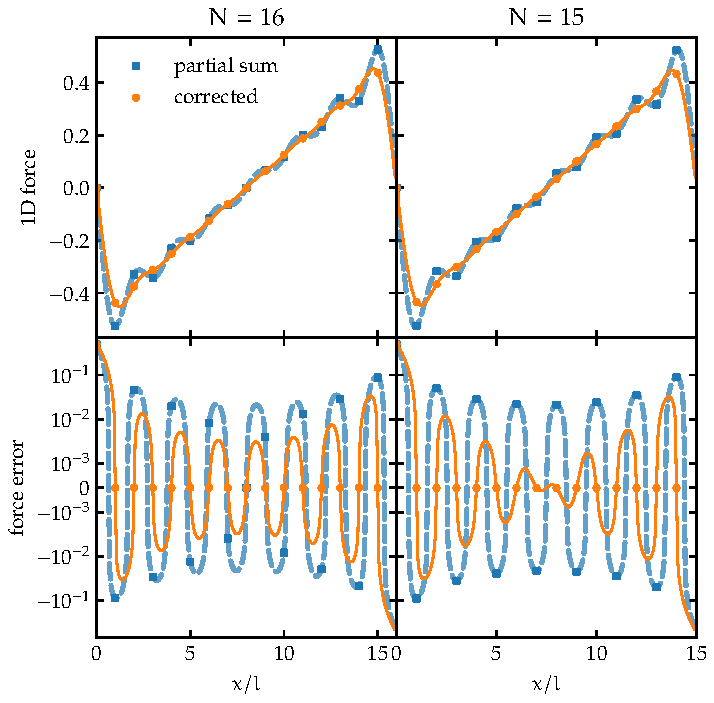
\includegraphics[width=0.7\linewidth]{force1D.pdf}
\caption{1D periodic forces with grids of even and odd lengths, from a
point source at $x=0$.}
\label{fig:force1D}
\end{figure*}


\subsubsection{Windowed partial sum?}

Consider the $p$-th order B-spline window in 1D,
%
\begin{equation}
W_p(k_n) = \biggl( \frac{\sin k_n l / 2}{k_n l / 2} \biggr)^p.
\end{equation}
%
When the particles are scattered to the mesh (see \autoref{sec:equiv})
using such a kernel, one usual practice is to approximately ``undo'' the
smearing by a deconvolution.
This is done by dividing the force by $W_p^2(k_n)$, with $W_p$ squared
because of the additional smearing when gathering the particle forces
from the mesh.
\st{
If we take the deconvolutions into account in modeling the partial sum
approximation, this will change the shape of the Dirichlet kernel.
However, we are not able to find the analytic expression of the new
kernel.
}


\YL{\st{Minimize force error above a certain radius, e.g. beyond 27 cells,
(in a way similar to choosing NUFFT kernel?)}:
\begin{itemize}
\item \url{https://arxiv.org/abs/1712.04732},
\item \url{https://www.frontiersin.org/articles/10.3389/fphy.2016.00028/full},
\item \url{https://journals.aps.org/pre/pdf/10.1103/PhysRevE.95.063303}.
\end{itemize}
}


\YL{Filter/window design: Jupyter notebook with interactive sliders,
\href{https://docs.scipy.org/doc/scipy/reference/signal.windows.html}{scipy.signal.windows},
\href{https://docs.scipy.org/doc/scipy/reference/signal.html}{scipy.signal}.
}


\YL{\st{2 possible ways to optimize:
suppress the oscillation outside of the PP patch size;
shift the phase of the oscillation so that there are both positive and
negative parts between two nearby mesh points.}
}


\subsubsection{Equivalent Point Source}
\label{sec:equiv}

simple cubic (CIC), bcc, interlocking/interlacing cubic.
\YL{See \cite{HockneyEastwood1988} for the interlacing one.
Other references:
\begin{itemize}
\item \url{https://aip.scitation.org/doi/10.1063/1.3430521},
\item \url{https://aip.scitation.org/doi/pdf/10.1063/1.3430521},
\item \url{https://aip.scitation.org/doi/pdf/10.1063/1.3657407}.
\end{itemize}
}

%* Suppose the two interlacing meshes are A and B, is the following a way
%  to have 16 equivalent grid points (up to octopole)?
%  1. src: (A + shifted B) at A, tgt: A
%  2. src: (B + shifted A) at B, tgt: B


\subsection{Particle-Particle Force}



\subsection{Force Patching}


\YL{Quantify force error including (position-dependent) magnitude and
volume.}


For cosmological applications, we want to optimize for point clouds that
are uniform (and Gaussian with known power spectrum) on large scales.


\subsection{Complexity}

$N$ particles, $M$ cells, volume $V$, mean matter density
$\bar\rho$, particle mass $m = \bar\rho V / N$, density field $\rho(\vx)
= \bar\rho [1 + \delta(\vx)]$, $C_i$ is the $i$-th cell, and $D_i$ are
the cells whose particles directly interact with those in $C_i$ (so $C_i
\subsetneq D_i$).
Each cell $C$ has volume $V / M$, and each direct interacting region $D$
has volume $d V / M$ with $d$ being an integer greater than 1.
The total number of pairs of interactions is
%
\begin{align}
\tsum_{i=1}^M \E \bigl[ \tsum_{p\in C_i} \1_{p'\in D_i} \bigr]
%
&\simeq \tsum_{i=1}^M \frac{N^2}{V^2}
  \int_{C_i} \!\!\!\d\vx \int_{D_i} \!\!\!\d\vx'\,
  \E \bigl\{ [1 + \delta(\vx)] [1 + \delta(\vx')] \bigr\} \nonumber\\
%
&= \frac{M N^2}{V^2} \int_C \!\!\d\vx \int_D \!\!\d\vx'\,
  \bigl[ 1 + \xi(\vx' - \vx) \bigr]
= \frac{d N^2}M  \bigl( 1 + \sigma^2_{CD} \bigr),
\end{align}
%
where $\xi$ is the matter density 2-point correlation function, and we
have replaced the sums over particles with the integrals over the
density fields, $\sum_p \to m^{-1} \int \!\d\vx\, \rho(\vx) = N V^{-1}
\int \!\d\vx\, [1 + \delta(\vx)]$, in deriving the first equality.
We have also used the density covariance between $C$ and $D$, defined as
%
\begin{equation}
\sigma^2_{CD} \triangleq \int \!\!\frac{\d\vk}{(2\pi)^3}\,
  P(k) W_C^*(\vk) W_D(\vk)
= \frac{M^2}{d V^2} \int_C \!\!\d\vx \int_D \!\!\d\vx'\,
  \xi(\vx' - \vx),
\end{equation}
%
where $P(k)$ is the matter density power spectrum and the Fourier
transform of $\xi$.
$\sigma^2_{CD}$ depends on the geometry of $C$ and $D$, through their
Fourier space windows:
%
\begin{align}
W_C(\vk) &\triangleq \frac{M}V \int_C \!\!\d\vx\, e^{i\vk\cdot\vx},
  \nonumber\\
W_D(\vk) &\triangleq \frac{M}{dV} \int_D \!\!\d\vx\, e^{i\vk\cdot\vx},
\end{align}
%
both normalized to 1 at $\vk=\vzero$.


\YL{Optimal mesh cell size given $\sigma^2_{CD}$ for fixed error budget,
cosmology and time dependence.}




\section{Results}


\section{Conclusions}






\bibliographystyle{plain}
\bibliography{pp}



\end{document}
